\begin{center}
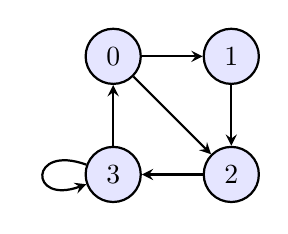
\begin{tikzpicture}[
  vnode/.style={circle, draw, minimum size=7mm, inner sep=0pt, fill=blue!10},
  thick,
  >=stealth
]
  \node[vnode] (0) at (0, 1.2) {0};
  \node[vnode] (1) at (1.5, 1.2) {1};
  \node[vnode] (2) at (1.5, -0.3) {2};
  \node[vnode] (3) at (0, -0.3) {3};
  
  \draw[->] (0) -- (1);
  \draw[->] (1) -- (2);
  \draw[->] (2) -- (3);
  \draw[->] (3) -- (0);
  \draw[->] (0) -- (2);
  \draw[->] (3) to [out=160, in=200, looseness=8] (3);
\end{tikzpicture}
\par\medskip
\textit{Obrázek 5.3: Příklad orientovaného grafu se smyčkou na vrcholu 3.}
\end{center}